\Titular%
{filosofia}%
{Somos donos das nosas decisións?}%
{Mauro Garrido Rodríguez}%
{Entre o determinismo clásico, a aleatoriadade cuántica e o <<eu>>.}%

\begin{multicols}{2}

\subsection*{Que é o libre arbitrio?}

Día a día experimentamos con claridade que somos donos das decisións que
tomamos conscientemente: cando digo \textit{<<vou dar un paseo>>}, mentalmente
fixen unha balanza de opcións e determineime por unha delas, é dicir, podo
afirmar, mirando cara ao pasado, que \textit{<<puiden non ter dado un paseo>>}.
Estar obrigado a dar un paseo é o oposto de ser libre. Así, dicimos:
\textit{<<Son libre se, tendo feito A e non B, puidese ter actuado de xeito
distinto e facer B no canto de A>>}. Lingüisticamente, esta é unha sentencia
contrafactual (\textit{contra os feitos}, contradicindo o que realmente
ocorreu), á que, como vimos, sempre lle damos validez (é dicir, que
consideramos verdadeira a posibilidade de poder contradici-los feitos nunha
realidade alternativa), polo que tamén é un \textbf{presuposto metafísico}.

\subsection*{A fin da liberdade: o demo de Laplace}

Pero, que di a física a respecto da validez deste suposto? O certo é que, se
consideramo-lo Universo a grande escala, e inclusive nas nosas vidas cotiás, a
mecánica clásica está no seu intervalo de validez. Que nos pode dicir sobre o
libre arbitrio? Collamo-las Leis de Newton. O que nos permiten é, coñecendo o
estado inicial dun sistema (é dicir, a posición e velocidade das partículas
involucradas), determina-lo seu estado futuro, de xeito que
%
\begin{equation}
    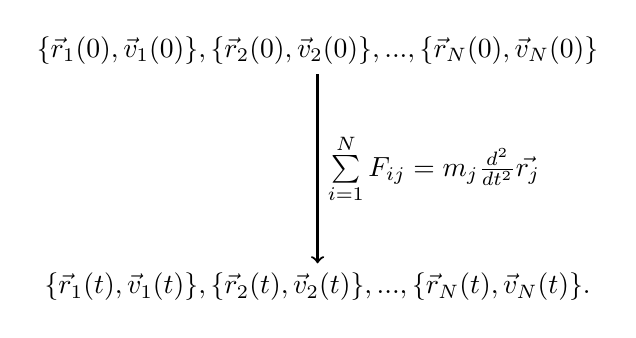
\begin{tikzpicture}[baseline=(current bounding box.center)]
        \node (A) at (0,0)
        {$
            \{ \vec{r}_1(0), \vec{v}_1(0)\},
            \{ \vec{r}_2(0), \vec{v}_2(0) \}, ... ,
            \{ \vec{r}_N (0), \vec{v}_N(0) \}
        $};
        \node (B) at (0,-3)
        {$
            \{ \vec{r}_1(t), \vec{v}_1(t)\},
            \{ \vec{r}_2(t), \vec{v}_2(t) \}, ... ,
            \{ \vec{r}_N(t), \vec{v}_N(t) \}.
        $};
        \draw[->, thick] (A) -- (B) node[midway,right]
        {$\sum\limits_{i=1}^N F_{ij} = m_j \large\frac{d^2}{dt^2}\vec{r_j}$};
    \end{tikzpicture}
\end{equation}
%
Isto é, se coñecemo-lo estado inicial con total precisión, tamén coñeceremos
con total exactitude o estado final, así como toda a dinámica en cada momento:
o futuro está contido no pasado. As leis de Newton son, polo tanto,
\textbf{deterministas causais}: cada causa leva univocamente a un efecto. E se
todo está composto de átomos, incluídos nós mesmos... Non aplicará isto tamén
ao ser humano? Isto é precisamente o que se preguntou Pierre-Simon Laplace en
$1814$, co seu famoso experimento mental do \textit{<<demo de Laplace>>} (pese
a que este nunca o chamou <<demo>>), onde expoñía o
seguinte\cite{wikidemolaplace}:

\textit{<<Un intelecto que nun momento determinado coñecese tódalas forzas que
moven a natureza e tódalas posicións de tódolos elementos que a compoñen, se
este intelecto fose o suficientemente vasto como para someter estes datos a
análise, abarcaría nunha soa fórmula os movementos dos corpos máis grandes do
Universo e os do átomo máis diminuto; para tal intelecto nada sería incerto, e
o futuro, ao igual que o pasado, podería estar presente ante os seus ollos.>>}

\begin{figure}[H]
    \centering
    \includegraphics[width=\linewidth]{revistas/004/imaxes/demo_laplace.png}
    \caption{Ilustración do Demo de Laplace\cite{demo_laplace}}
    \label{demo_laplace}
\end{figure}

Segundo este experimento mental, cada acto, cada movemento, cada pensamento e
cada decisión transcendental que puidésemos facer, sería coñecido polo demo: en
esencia non habería diferenza entre as nosas vidas e as bólas nunha partida de
billar, todo estaría predeterminado dende o inicio.

\subsection*{A contradición coa nosa experiencia inmediata}

Por suposto, non vivimos coma se o demo de Laplace existise. Día a día
experimentamos coa máxima claridade posible que somos libres e que somos donos
das nosas decisións, polo que algo nos escapa. Un xeito de entender isto é que
quizais poidamos seguir dicindo que somos libres nun universo determinista se
nos contentamos cunha liberdade menos metafísica e fundamental, dicindo:
\textit{<<Son libre (ou teño libre arbitrio) se podo actuar baixo os meus
propios desexos e razóns, sen estar sometido á coacción externa>>}. É certo
que, visto dende o punto de vista metafísico, esta liberdade sabe a pouco: que
esteamos coaccionados ou non, incluso os nosos propios desexos, xa sería algo
predeterminado e, polo tanto, algo que non podemos cambiar (se o Universo
funciona de xeito determinista). Pero, se descoñecemos esta información, se non
falamos co demo, acaso non podemos dicir que somos libres en certo senso?

Nas nosas sociedades humanas o concepto de libre arbitrio é totalmente
fundamental. Existe a responsabilidade se todo está determinado dende o
principio? Como se pode condenar alguén por un delito cando xa estaba escrito
que cometería ese delito? Por suposto, o determinismo absoluto fai da
responsabilidade un absurdo: incluso a decisión sobre que sistema xudicial usar
e se basealo ou non no concepto de liberdade estaría tamén determinada. Este
artigo especulando acerca da imposibilidade do libre arbitrio tamén o estaría.

\subsection*{O indeterminismo esencial: é a Mecánica Cuántica a solución?}

Imos continuar a falar deste concepto de libre arbitrio máis metafísico, pese a
que tamén hai moito máis que dicir da posibilidade de liberdade nun mundo
estritamente determinista: o exposto brevemente aquí non é a última palabra,
por suposto.

O certo é que o determinismo (ou o \textit{universo mecánico}), como paradigma
científico, acumulaba éxito tras éxito en tódalas ciencias: a natureza
comportábase como un inmenso reloxo, onde era só a nosa ignorancia o que nos
impedía ve-lo movemento de tódalas pezas do mecanismo.

Pero claro está, chegou o século $XX$ e con el, a Mecánica Cuántica: o mundo
non sería nunca máis o mesmo, e a nosa concepción del, tampouco. A Cuántica
demóstranos que existe unha indeterminación, unha aleatoriedade a nivel
fundamental na natureza: non pola nosa ignorancia, senón debido a como
\textit{é}. O único determinismo que a Cuántica nos concede é un de
probabilidades, un que non é causal: unha mesma causa pode producir diferentes
efectos, aínda que podemos saber exactamente como as probabilidades de cada
efecto evolucionan co tempo a través da ecuación de Schrödinger:

\begin{equation}
    \Psi (0) \xrightarrow{\displaystyle i\hbar\frac{\partial \Psi}{\partial t} =
    \hat{H} \Psi} \Psi(t)
\end{equation}

Pero o que nos di é que, en esencia, a natureza é aleatoria. Entón, realmente a
cuántica danos liberdade co seu carácter aleatorio, asumindo que xoga algún
rol, por pequeno que sexa, no noso cerebro (nun sistema tan grande e quente non
agardariamos fenómenos cuánticos en principio)? Xa o estamos dicindo: é algo
aleatorio. É como dicir que, ante a decisión de mover ou non o brazo para
coller un vaso, esta fose totalmente determinada polo resultado de cara ou cruz
dun lanzamento de moeda (considerando o lanzamento como un proceso totalmente
aleatorio). Non sabemos que resultado sairá nin é algo que estea determinado,
mais, é isto o que chamamos decidir por nós mesmos? Polo tanto, a Cuántica
tampouco nos dá ese libre arbitrio metafísico que andamos buscando.

\begin{figure}[H]
    \centering
    \includegraphics[width=\linewidth]{revistas/004/imaxes/schrodinger_santiago.jpg}
    \caption{Schrödinger en Santiago de Compostela, 1934\cite{wikidemolaplace}}
    \label{schrodinger_santiago}
\end{figure}

\subsection*{O \textit{<<eu>>} que escapa ao Universo}

Se nos detemos un momento, parécese intuír algo: todo o que somos son causas
externas. A que nos referimos cando queremos afirmar \textit{<<eu son libre>>}?
Que queda do \textit{<<eu>>} se subtraemos de nós a xenética, as condicións
sociais, o noso pasado... Parecese que, para sermos libres, precisásemos ser
alleos ao Universo, escapar incluso da limitación que nos impón segui-las súas
leis; como ben diría Schrödinger:\cite{queeavida}

\textit{<<Eu>>--- son a persoa, se é que existe algunha, que controla o
<<movemento dos átomos>>, de acordo coas leis da Natureza.}

Así, se quixésemos afirmar que o ser humano é metafisicamente libre, teriamos
que chegar ao extremo de dicir que ten algo que o fai esencialmente diferente
ao resto de corpos no Universo, que ten que sobreporse incluso ás leis que o
rexen e dirixir segundo as leis naturais os mesmos átomos que o compoñen,
afirmar, en definitiva, \textit{<<Polo tanto, eu son Deus
Todopoderoso>>}.\cite{queeavida}

\nocite{wikidemolaplace}

\printbibliography

\end{multicols}
